\chapter{Statistika Pengukuran Kimia}\label{ch:b2:measurement-statistics}

Dua laboratorium mengukur timbal dalam air keran yang sama dan melaporkan
9.6 dan \qty{11.2}{\micro g/L}. Nilai pedoman untuk air minum adalah
\qty{10}{\micro g/L}. Apakah air itu layak diminum? Apakah kedua laboratorium
itu benar-benar berbeda pendapat, ataukah kedua hasil itu adalah nilai yang
sama yang terlihat melalui sebaran dua pengukuran? Bilangan hasil analisis
tidak berarti apa-apa tanpa ketidakpastiannya, dan bab ini memberikan
alat-alat untuk menghitungnya: statistika pengukuran berulang, perambatan
ketidakpastian melalui sebuah perhitungan, kalibrasi dengan kuadrat
terkecil, dan batas-batas yang di bawahnya sebuah metode tidak melihat apa
pun.
% ledger: who:lead

\begin{omfigure}
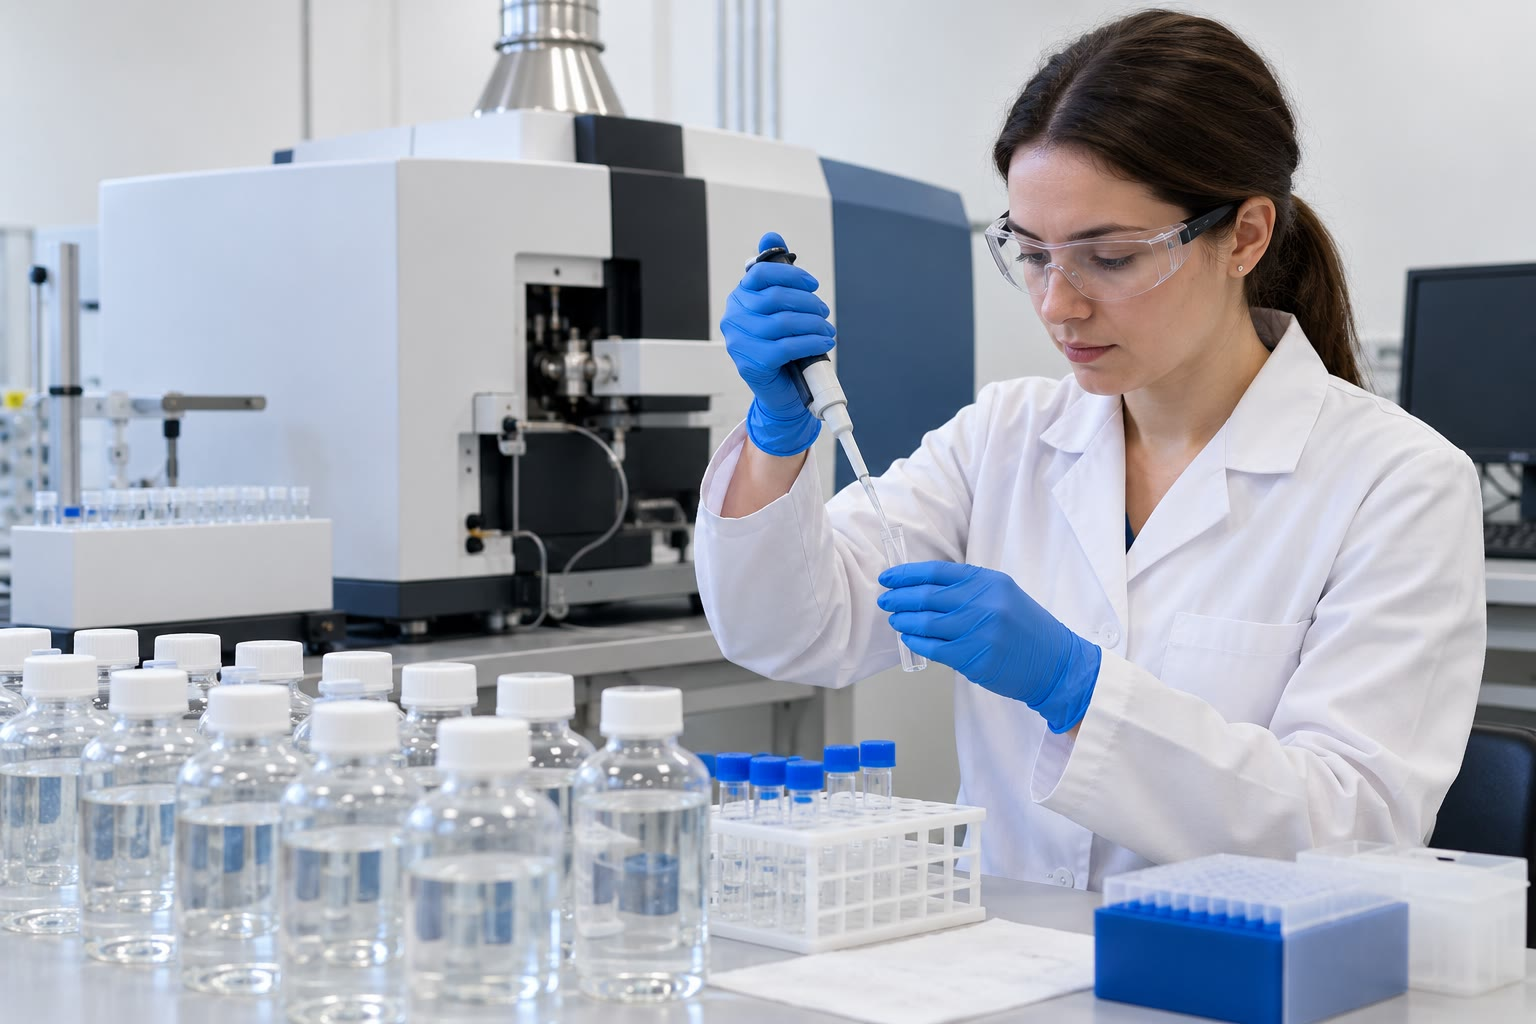
\includegraphics[width=0.56\linewidth]{images/book3/ai/b2-34-water-lab.jpg}

{\small Sebuah laboratorium pengujian air: botol-botol sampel, seorang teknisi
yang memipet, sebuah penganalisis unsur di belakang (ilustrasi).}
\end{omfigure}

\begin{recall}
Jilid Tahun 1: ketidakpastian pengukuran, ketidakpastian baku, evaluasi
tipe A dan tipe B, ketidakpastian diperluas, ketidakpastian relatif, deviasi
ternormalisasi $z$ antara dua nilai, dan janji akan bukti $u(\bar x) = s/\sqrt n$
serta aturan perambatan yang umum. Jilid sekolah: garis kalibrasi.
\Cref{ch:b2:mass-spec-atomic}: serapan atom.
\end{recall}

\section{Pengukuran berulang}

Ulangilah sebuah pengukuran, maka hasil-hasilnya tersebar. Setiap hasil
$x_i$ diperlakukan sebagai variabel acak dengan rerata $\mu$ (nilai yang
rata-rata akan diberikan oleh metode itu) dan simpangan baku $\sigma$; jika
banyak penyebab kecil yang saling bebas menjumlah, hasil-hasilnya mengikuti
hukum normal (Gauss), dengan sekitar 68~\% di antaranya
dalam $\mu \pm \sigma$ dan 95~\% dalam $\mu \pm 1.96\sigma$.

\begin{definition}[Dispersi]\label{def:b2:measurement-statistics:dispersion}
Untuk $n$ hasil $x_1, \dots, x_n$ dengan rerata $\bar x$, \emph{simpangan baku
eksperimental}\index{simpangan baku eksperimental} adalah
$s = \sqrt{\sum (x_i - \bar x)^2/(n-1)}$; besaran ini menaksir $\sigma$.
Yang disebut \emph{simpangan baku rerata}\index{simpangan baku rerata}
adalah simpangan baku $\bar x$ pada banyak deret $n$ hasil, yang ditaksir
dengan $s/\sqrt n$.
\end{definition}

Pembagi $n - 1$ alih-alih $n$ mengoreksi kenyataan bahwa simpangan-simpangan
diambil dari $\bar x$, yang dihitung dari data yang sama, sehingga
simpangan-simpangan itu sedikit terlalu kecil: $n - 1$ adalah banyaknya
simpangan yang saling bebas, yaitu derajat kebebasan.

\begin{theorem}[Variansi rerata]\label{thm:b2:measurement-statistics:mean-variance}
Jika $x_1, \dots, x_n$ saling bebas, masing-masing dengan variansi $\sigma^2$, maka $\operatorname{var}(\bar x) =
\sigma^2/n$: \omterm{def:b2:measurement-statistics:dispersion}{simpangan baku rerata} adalah $\sigma/\sqrt n$.
\end{theorem}

\begin{proof}
Untuk variabel-variabel yang saling bebas, variansi sebuah jumlah adalah
jumlah variansi-variansinya, dan
$\operatorname{var}(cX) = c^2\operatorname{var}(X)$. Jadi $\operatorname{var}(\bar x) =
\operatorname{var}\bigl(\tfrac1n\sum x_i\bigr) = \tfrac{1}{n^2}\sum\operatorname{var}(x_i) =
\tfrac{1}{n^2}\,n\sigma^2 = \sigma^2/n$. Mengganti $\sigma$ dengan taksirannya
$s$ menghasilkan ketidakpastian baku tipe A
$u(\bar x) = s/\sqrt n$ yang diterima tanpa bukti dalam jilid Tahun 1.
\end{proof}

\section{Selang kepercayaan}

\begin{definition}[Selang kepercayaan]\label{def:b2:measurement-statistics:confidence}
Yang disebut \emph{selang kepercayaan}\index{selang kepercayaan} pada
\emph{tingkat kepercayaan}\index{tingkat kepercayaan}
$1 - \alpha$ (sering 95~\%) adalah selang yang dihitung dari data dengan
sebuah aturan yang, jika diterapkan pada banyak deret, memuat nilai
sebenarnya pada fraksi $1 - \alpha$ dari deret-deret itu. Untuk rerata $n$
hasil, selang itu adalah $\bar x \pm t\,s/\sqrt n$, dengan $t$
\emph{koefisien Student}\index{koefisien Student}
untuk $n - 1$ derajat kebebasan dan tingkat itu.
\end{definition}

\begin{proposition}[Hukum Student]\label{prop:b2:measurement-statistics:student}
Untuk $n$ hasil normal yang saling bebas, $T = (\bar x - \mu)/(s/\sqrt n)$
mengikuti hukum Student dengan
$n - 1$ derajat kebebasan, yang kerapatannya sebanding dengan $(1 + t^2/\nu)^{-(\nu+1)/2}$ dengan
$\nu = n - 1$. Hukum ini lebih lebar daripada hukum normal dan mendekatinya
ketika $n$ bertambah.
\end{proposition}

\admitted

Membagi dengan $s$ alih-alih dengan $\sigma$ yang tidak diketahui
menambahkan sebaran $s$ itu sendiri, yang besar jika $n$ kecil; karena itu
ekor-ekornya lebih tebal, dan koefisien-koefisiennya lebih besar daripada
1.96. Tabel memberikan koefisien
95~\%, yang dihitung dari kerapatannya.

\begin{omfigure}
\begin{minipage}[c]{0.56\linewidth}
\begin{tikzpicture}
\begin{axis}[width=\linewidth, height=4.8cm, xmin=-5, xmax=5, ymin=0, ymax=0.43,
  xlabel={$t$}, ylabel={kerapatan}, label style={font=\small}, tick label style={font=\scriptsize},
  legend style={font=\scriptsize, at={(0.98,0.98)}, anchor=north east}, legend cell align=left]
\addplot[omThm, thick] table[x=t, y=nu2] {figdata/out/bachelor-2-regression-c.dat};
\addplot[omMeth, thick] table[x=t, y=nu5] {figdata/out/bachelor-2-regression-c.dat};
\addplot[black, thick, dashed] table[x=t, y=normal] {figdata/out/bachelor-2-regression-c.dat};
\legend{$\nu = 2$, $\nu = 5$, normal}
\end{axis}
\end{tikzpicture}
\end{minipage}\hfill
\begin{minipage}[c]{0.4\linewidth}\centering
\small
\begin{tabular}{rr}
\hline
$\nu = n - 1$ & $t$ (95~\%) \\
\hline
1 & 12.706 \\
2 & 4.303 \\
3 & 3.182 \\
4 & 2.776 \\
5 & 2.571 \\
9 & 2.262 \\
20 & 2.086 \\
$\infty$ & 1.960 \\
\hline
\end{tabular}
\end{minipage}
\par\vspace{4pt}

{\small Kerapatan Student untuk 2 dan 5 derajat kebebasan dibandingkan dengan
hukum normal, serta koefisien dua sisi
95~\%, yang dihitung dengan mengintegralkan kerapatannya (baris terakhir
adalah hukum normal).}
% figdata: bachelor-2/regression.py parts c, e
\end{omfigure}

\begin{method}[Selang kepercayaan untuk sebuah rerata]\label{met:b2:measurement-statistics:confidence-interval}
\begin{enumerate}
  \item Hitunglah $\bar x$ dan $s$ dari $n$ hasil; periksalah bahwa tidak
        ada hasil yang sangat menyimpang.
  \item Bacalah $t$ untuk $\nu = n - 1$ pada tingkat yang dipilih.
  \item Laporkan $\bar x \pm t\,s/\sqrt n$, dengan ketidakpastian yang
        dibulatkan sampai satu atau dua angka penting dan reratanya sampai
        tempat desimal yang sama.
  \item Untuk membandingkan dengan nilai acuan $x_{\mathrm{ref}}$, hitunglah $|\bar x - x_{\mathrm{ref}}|/(s/\sqrt
        n)$: di atas $t$, perbedaannya bermakna pada tingkat itu; di bawahnya,
        data tidak memperlihatkan perbedaan (yang tidak membuktikan bahwa
        perbedaan itu tidak ada).
\end{enumerate}
\end{method}

\section{Perambatan ketidakpastian}

\begin{theorem}[Hukum perambatan ketidakpastian]\label{thm:b2:measurement-statistics:propagation}
Jika $y = f(x_1, \dots, x_n)$, dengan $x_i$ saling bebas dan ketidakpastian
bakunya $u(x_i)$ cukup kecil sehingga $f$ hampir linear pada rentang itu,
maka
\begin{equation*}
u^2(y) = \sum_{i=1}^{n}\left(\frac{\partial f}{\partial x_i}\right)^2 u^2(x_i).
\end{equation*}
\end{theorem}

\begin{proof}
Sampai orde pertama (Taylor), $y - f(\mu_1, \dots, \mu_n) \approx \sum c_i(x_i - \mu_i)$ dengan $c_i = \partial
f/\partial x_i$ pada rerata-reratanya. Variansi kombinasi linear
variabel-variabel yang saling bebas adalah
$\sum c_i^2\operatorname{var}(x_i)$ (seperti pada \cref{thm:b2:measurement-statistics:mean-variance}); dengan
$\operatorname{var}(x_i) = u^2(x_i)$ inilah hasilnya.
\end{proof}

\begin{corollary}[Jumlah dan hasil kali]\label{cor:b2:measurement-statistics:products}
Untuk jumlah atau selisih, ketidakpastian-ketidakpastian baku menjumlah
secara kuadratur: $u^2(x_1 \pm x_2) = u^2(x_1) +
u^2(x_2)$. Untuk hasil kali atau hasil bagi $y = x_1^{a}x_2^{b}\cdots$,
ketidakpastian-ketidakpastian relatif menjumlah secara kuadratur,
masing-masing berbobot pangkatnya: $\bigl(u(y)/y\bigr)^2 = a^2\bigl(u(x_1)/x_1\bigr)^2 +
b^2\bigl(u(x_2)/x_2\bigr)^2 + \cdots$
\end{corollary}

\begin{proof}
Untuk jumlah, turunan-turunan parsialnya adalah $\pm1$. Untuk $y = x_1^ax_2^b$, $\partial y/\partial x_1 =
a\,y/x_1$ dan $\partial y/\partial x_2 = b\,y/x_2$; teorema itu memberikan $u^2(y) = a^2y^2u^2(x_1)/x_1^2 +
b^2y^2u^2(x_2)/x_2^2$; bagilah dengan $y^2$.
\end{proof}

\begin{method}[Merambatkan ketidakpastian]\label{met:b2:measurement-statistics:propagate}
\begin{enumerate}
  \item Tuliskan hasilnya sebagai rumus besaran-besaran yang diukur;
        daftarlah setiap masukan beserta ketidakpastian bakunya (tipe A atau B).
  \item Untuk hasil kali dan hasil bagi, bekerjalah dengan ketidakpastian
        relatif; untuk jumlah, dengan ketidakpastian mutlak; selain itu,
        ambillah turunan parsial.
  \item Gabungkan secara kuadratur; temukan suku yang dominan: memperbaiki
        suku-suku lain adalah upaya yang sia-sia.
  \item Kalikan dengan faktor cakupan (2, atau $t$ Student jika suku yang
        dominan berasal dari sedikit ulangan) untuk memperoleh
        ketidakpastian diperluas.
\end{enumerate}
\end{method}

\section{Kalibrasi}

\begin{definition}[Kurva kalibrasi]\label{def:b2:measurement-statistics:calibration}
Yang disebut \emph{kurva kalibrasi}\index{kurva kalibrasi} menghubungkan
sinyal $y$ sebuah instrumen dengan
konsentrasi $x$, dari standar-standar yang konsentrasinya diketahui. Yang
disebut \emph{garis kuadrat
terkecil}\index{garis kuadrat terkecil} $y = a + bx$ adalah garis yang meminimumkan $S = \sum (y_i - a -
bx_i)^2$; setiap $e_i = y_i - a - bx_i$ adalah sebuah \emph{sisaan}\index{sisaan}.
\end{definition}

\begin{theorem}[Garis kuadrat terkecil]\label{thm:b2:measurement-statistics:least-squares}
Dengan $\bar x$, $\bar y$ rerata-reratanya, $S_{xx} = \sum(x_i - \bar x)^2$ dan $S_{xy} = \sum(x_i - \bar x)(y_i -
\bar y)$, \omterm{def:b2:measurement-statistics:calibration}{garis kuadrat terkecil} mempunyai
\begin{equation*}
b = \frac{S_{xy}}{S_{xx}}, \qquad a = \bar y - b\bar x.
\end{equation*}
\end{theorem}

\begin{proof}
$S$ adalah fungsi kuadrat dari $a$ dan $b$. Turunan-turunan parsialnya
bernilai nol pada minimum:
$\partial S/\partial a = -2\sum(y_i - a - bx_i) = 0$ memberikan $a = \bar y - b\bar x$; menyubstitusikannya ke dalam
$\partial S/\partial b = -2\sum x_i(y_i - a - bx_i) = 0$ memberikan $\sum x_i\bigl((y_i - \bar y) - b(x_i -
\bar x)\bigr) = 0$, yaitu $S_{xy} = bS_{xx}$ (karena $\sum \bar x(y_i - \bar y) = \sum \bar x(x_i - \bar
x) = 0$). Turunan-turunan keduanya membentuk matriks
\[\begin{pmatrix} 2n & 2\sum x_i\\ 2\sum x_i & 2\sum x_i^2\end{pmatrix},\]
yang diagonalnya positif dan determinannya $4nS_{xx}$ positif jika $x_i$
tidak semuanya sama: titik stasionernya adalah minimum.
\end{proof}

\begin{proposition}[Membaca sebuah konsentrasi]\label{prop:b2:measurement-statistics:interpolation}
Untuk $n$ standar dengan simpangan baku \omterm{def:b2:measurement-statistics:calibration}{sisaan} $s_{y/x} = \sqrt{\sum e_i^2/(n-2)}$,
sampel yang dibaca
$m$ kali dengan sinyal rata-rata $\bar y_0$ mempunyai $x_0 = (\bar y_0 - a)/b$ dan simpangan baku
\begin{equation*}
s_{x_0} = \frac{s_{y/x}}{b}\sqrt{\frac1m + \frac1n + \frac{(\bar y_0 - \bar y)^2}{b^2S_{xx}}},
\end{equation*}
yang dipakai bersama $t$ Student untuk $n - 2$ derajat kebebasan.
\end{proposition}

\admitted

Ketiga suku di bawah tanda akar adalah sebaran pembacaan sampel,
ketidakpastian tinggi garis, dan ketidakpastian kemiringannya; suku
terakhir lenyap di tengah rentang kalibrasi, yaitu tempat sampel paling
baik dibaca.

\begin{omfigure}
\begin{tikzpicture}
\begin{axis}[width=0.5\linewidth, height=5cm, xmin=-1, xmax=22, ymin=0, ymax=0.22,
  xlabel={timbal (\unit{\micro g/L})}, ylabel={absorbans}, label style={font=\small},
  tick label style={font=\scriptsize}, scaled y ticks=false,
  yticklabel style={/pgf/number format/fixed, /pgf/number format/precision=2}]
\addplot[omDef, thick] table[x=x, y=line] {figdata/out/bachelor-2-regression-b.dat};
\addplot[only marks, mark=*, mark size=1.8pt, omThm] table[x=x, y=A] {figdata/out/bachelor-2-regression-a.dat};
\end{axis}
\end{tikzpicture}\hfill
\begin{tikzpicture}
\begin{axis}[width=0.5\linewidth, height=5cm, xmin=-1, xmax=22, ymin=-0.002, ymax=0.002,
  xlabel={timbal (\unit{\micro g/L})}, ylabel={sisaan}, label style={font=\small},
  tick label style={font=\scriptsize}, scaled y ticks=false, ycomb,
  yticklabel style={/pgf/number format/fixed, /pgf/number format/precision=3},
  extra y ticks={0}, extra y tick style={grid=major, grid style={black!50}}]
\addplot[omThm, thick, mark=*, mark size=1.6pt] table[x=x, y=res] {figdata/out/bachelor-2-regression-a.dat};
\end{axis}
\end{tikzpicture}

{\small Kalibrasi timbal dengan serapan atom tanur grafit pada
\qty{283.3}{nm} (data latihan, dipakai dalam soal). Kiri: kelima standar
dan \omterm{def:b2:measurement-statistics:calibration}{garis kuadrat terkecil}. Kanan: \omterm{def:b2:measurement-statistics:calibration}{sisaan-sisaannya}, kecil dan tanpa pola:
garis lurus sudah memadai.}
% figdata: bachelor-2/regression.py parts a, b
% ledger: asd:Pb283
\end{omfigure}

\begin{method}[Mengalibrasi]\label{met:b2:measurement-statistics:calibrate}
\begin{enumerate}
  \item Siapkan lima standar atau lebih yang mencakup rentang yang
        diperkirakan, dalam matriks yang sama dengan sampel, dan sebuah
        blangko.
  \item Cocokkan \omterm{def:b2:measurement-statistics:calibration}{garis kuadrat terkecil}; alurkan \omterm{def:b2:measurement-statistics:calibration}{sisaan-sisaannya}. Pola yang
        melengkung berarti tanggapannya tidak linear: persempit rentangnya
        atau cocokkan sebuah kurva. Satu \omterm{def:b2:measurement-statistics:calibration}{sisaan} yang besar menunjuk pada
        standar yang keliru.
  \item Bacalah sampel-sampel, sebaiknya di dekat tengah rentang, secara
        berulang; hitunglah $x_0$ dan
        $s_{x_0}$.
  \item Laporkan $x_0 \pm t\,s_{x_0}$ setelah mengoreksi setiap pengenceran,
        dengan menambahkan ketidakpastian pengenceran yang dirambatkan jika
        tidak dapat diabaikan.
\end{enumerate}
\end{method}

\begin{definition}[Adisi standar]\label{def:b2:measurement-statistics:standard-addition}
Dalam \emph{metode adisi standar}\index{metode adisi standar}, sejumlah
analit yang diketahui ditambahkan ke porsi-porsi sampel itu sendiri yang
sama besar; sinyal dialurkan terhadap konsentrasi yang ditambahkan, dan
konsentrasi analit dalam sampel adalah jarak dari titik asal ke titik
tempat garis yang diekstrapolasi ke sinyal nol memotong sumbu, $a/b$.
\end{definition}

\begin{method}[Adisi standar]\label{met:b2:measurement-statistics:standard-addition}
\begin{enumerate}
  \item Pakailah metode ini jika matriks sampel mengubah tanggapan (garam,
        asam, bahan organik), sehingga standar dalam air murni akan
        memberikan kemiringan yang salah.
  \item Tambahkan sejumlah analit yang diketahui dan makin besar ke
        porsi-porsi yang sama, encerkan semuanya sampai volume yang sama,
        lalu ukurlah.
  \item Cocokkan garisnya; konsentrasi dalam larutan yang diukur adalah
        $a/b$; koreksilah pengencerannya.
  \item Tanggapannya harus linear sejak nol: periksalah \omterm{def:b2:measurement-statistics:calibration}{sisaan-sisaannya}.
\end{enumerate}
\end{method}

\begin{omfigure}
\begin{tikzpicture}
\begin{axis}[width=0.62\linewidth, height=5cm, xmin=-4, xmax=7, ymin=0, ymax=0.42,
  xlabel={konsentrasi yang ditambahkan (\unit{mg/L})}, ylabel={absorbans}, label style={font=\small},
  tick label style={font=\scriptsize}, axis lines=left, scaled y ticks=false,
  yticklabel style={/pgf/number format/fixed, /pgf/number format/precision=1}]
\draw[black!40] (axis cs:0,0) -- (axis cs:0,0.42);
\addplot[omDef, thick, densely dashed] table[x=x, y=line] {figdata/out/bachelor-2-regression-d-line.dat};
\addplot[only marks, mark=*, mark size=1.8pt, omThm] table[x=x, y=A] {figdata/out/bachelor-2-regression-d.dat};
\draw[<->, omMeth, thick] (axis cs:-3.11,0.06) -- (axis cs:0,0.06); \node[omMeth, below, font=\scriptsize] at (axis cs:-0.8,0.055) {$a/b$};
\end{axis}
\end{tikzpicture}

{\small Adisi standar (data latihan): absorbans sampel yang ditambahi 0, 2,
4, dan
\qty{6}{mg/L} analit. Garisnya memotong sinyal nol pada \qty{-3.11}{mg/L}:
larutan yang diukur mengandung \qty{3.11}{mg/L}.}
% figdata: bachelor-2/regression.py part d
\end{omfigure}

\section{Deteksi, kuantifikasi, dan validasi}

\begin{definition}[Batas]\label{def:b2:measurement-statistics:limits}
Yang disebut \emph{batas deteksi}\index{batas deteksi} sebuah metode adalah
konsentrasi terkecil yang sinyalnya dapat dibedakan dari sinyal blangko
dengan risiko deteksi palsu yang kecil dan dinyatakan; \emph{batas
kuantifikasi}\index{batas kuantifikasi} adalah konsentrasi terkecil yang
dapat diukur dengan ketidakpastian relatif yang dapat diterima.
\end{definition}

\begin{proposition}[Taksiran yang lazim]\label{prop:b2:measurement-statistics:lod}
Dengan $s_{\mathrm{blank}}$ simpangan baku sinyal-sinyal blangko berulang
dan $b$ kemiringan garis kalibrasi,
$x_{\mathrm{LOD}} \approx 3s_{\mathrm{blank}}/b$ dan $x_{\mathrm{LOQ}} \approx
10s_{\mathrm{blank}}/b$.
\end{proposition}

\begin{proof}[Argumen]
Jika sinyal-sinyal blangko normal dengan simpangan baku $s_{\mathrm{blank}}$,
sebuah blangko melampaui reratanya lebih dari $3s_{\mathrm{blank}}$ dengan
peluang sekitar 0.13~\% (ekor satu sisi hukum normal di luar
3 simpangan baku): menyebut sebuah sinyal ``terdeteksi'' di atas ambang itu
jarang mengira blangko sebagai sampel. Sinyal yang $10s_{\mathrm{blank}}$ di
atas blangko mempunyai simpangan baku relatif sekitar
10~\%, ambang lazim untuk hasil kuantitatif. Membagi dengan $b$ mengubah
sinyal menjadi konsentrasi.
\end{proof}

\begin{definition}[Validasi]\label{def:b2:measurement-statistics:validation}
Yang disebut \emph{kebenaran}\index{kebenaran} adalah kedekatan rerata
sejumlah besar hasil dengan nilai sebenarnya; selisih keduanya adalah
\emph{bias}\index{bias}. Yang disebut \emph{presisi}\index{presisi} adalah
kedekatan hasil-hasil yang saling bebas satu sama lain, yang dinyatakan
sebagai simpangan baku: \emph{keterulangan}\index{keterulangan} dalam
kondisi yang sama (operator, instrumen, laboratorium yang sama, dalam waktu
singkat), \emph{ketertiruan}\index{ketertiruan} dalam kondisi yang berubah
(laboratorium yang berbeda). Yang disebut \emph{validasi
metode}\index{validasi metode} adalah himpunan percobaan yang menetapkan,
untuk sebuah metode, kebenaran, presisi, kelinearan dan rentangnya, serta
\omterm{def:b2:measurement-statistics:limits}{batas deteksi} dan \omterm{def:b2:measurement-statistics:limits}{batas kuantifikasinya}.
\end{definition}

\omterm{def:b2:measurement-statistics:validation}{Kebenaran} diperiksa terhadap bahan acuan bersertifikat atau dengan
penambahan analit; \omterm{def:b2:measurement-statistics:validation}{presisi} diperiksa dengan ulangan dalam satu laboratorium
dan dengan perbandingan antarlaboratorium. Sebuah metode dapat presisi
tetapi \omterm{def:b2:measurement-statistics:validation}{bias}, dengan setiap hasil dekat dengan hasil lainnya dan semuanya
salah: \omterm{def:b2:measurement-statistics:validation}{presisi} bukanlah bukti \omterm{def:b2:measurement-statistics:validation}{kebenaran}.

\begin{history}[Student, 1908]
\begin{minipage}[t]{0.17\linewidth}
\vspace{0pt}
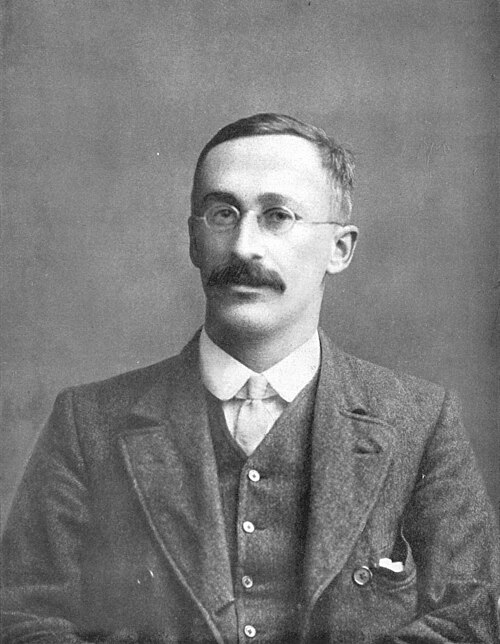
\includegraphics[width=\linewidth]{images/book3/gosset.jpg}
\end{minipage}\hfill
\begin{minipage}[t]{0.79\linewidth}
\vspace{0pt}
William Sealy Gosset, seorang kimiawan yang bekerja untuk sebuah pabrik bir,
harus menilai bahan baku dari sampel yang sangat sedikit, terlalu sedikit
untuk hukum normal. Pada tahun 1908 ia menerbitkan sebaran rerata dibagi
simpangan baku sampel, dengan nama samaran ``Student'' karena majikannya
tidak mengizinkan staf menerbitkan dengan nama sendiri. Hukum Student
dipakai setiap kali seorang analis menyebutkan selang dari tiga atau empat
ulangan. (Foto, 1908: domain publik; Wikimedia Commons.)
\end{minipage}
\end{history}

\section{Latihan}

\begin{exercise}[$\star$]\label{exo:b2:measurement-statistics:1}
Lima titrasi memberikan 12.45, 12.50, 12.48, 12.52, dan \qty{12.46}{mL}.
Hitunglah rerata, \omterm{def:b2:measurement-statistics:dispersion}{simpangan baku eksperimental}, dan \omterm{def:b2:measurement-statistics:dispersion}{simpangan baku
reratanya}.
\end{exercise}

\begin{exercise}[$\star$]\label{exo:b2:measurement-statistics:2}
Tuliskan \omterm{def:b2:measurement-statistics:confidence}{selang kepercayaan} 95~\% rerata pada latihan~1.
\end{exercise}

\begin{exercise}[$\star$]\label{exo:b2:measurement-statistics:3}
Sebuah larutan dibuat dengan melarutkan $m = \qty{0.5000}{g}$ ($u = \qty{0.0002}{g}$)
sebuah padatan dalam labu
$V = \qty{250.0}{mL}$ ($u = \qty{0.15}{mL}$). Hitunglah ketidakpastian baku
relatif $c = m/(MV)$, dengan massa molar yang cukup eksak.
\end{exercise}

\begin{exercise}[$\star$]\label{exo:b2:measurement-statistics:4}
Cocokkan \omterm{def:b2:measurement-statistics:calibration}{garis kuadrat terkecil} melalui $(0, 0.02)$, $(1, 0.21)$, $(2, 0.39)$, $(3, 0.62)$.
\end{exercise}

\begin{exercise}[$\star\star$]\label{exo:b2:measurement-statistics:5}
Sebuah larutan acuan bersertifikat mengandung \qty{10.00}{mg/L} sebuah
unsur. Lima analisis memberikan rerata
\qty{10.12}{mg/L} dengan $s = \qty{0.08}{mg/L}$. Apakah metode itu \omterm{def:b2:measurement-statistics:validation}{bias} pada tingkat 95~\%?
\end{exercise}

\begin{exercise}[$\star\star$]\label{exo:b2:measurement-statistics:6}
Konsentrasi ion hidronium diketahui dengan ketidakpastian baku relatif 2~\%.
Berapa ketidakpastian baku pH-nya?
\end{exercise}

\begin{exercise}[$\star\star$]\label{exo:b2:measurement-statistics:7}
Sepuluh blangko mempunyai $s = 0.0012$ satuan absorbans; kemiringan
kalibrasinya \qty{0.0098}{L/\micro g}. Perkirakan \omterm{def:b2:measurement-statistics:limits}{batas deteksi} dan \omterm{def:b2:measurement-statistics:limits}{batas
kuantifikasinya}.
\end{exercise}

\begin{exercise}[$\star\star$]\label{exo:b2:measurement-statistics:8}
Dalam percobaan adisi standar pada gambar, keempat porsi dibuat dengan
mengencerkan
\qty{10.0}{mL} sampel menjadi \qty{50.0}{mL}. Tentukan konsentrasi dalam sampel.
\end{exercise}

\begin{exercise}[$\star\star$]\label{exo:b2:measurement-statistics:9}
Dalam sebuah kajian antarlaboratorium, setiap laboratorium memperoleh
$s = \qty{0.05}{mg/L}$ pada ulangan-ulangannya sendiri, tetapi hasil
laboratorium-laboratorium yang berbeda tersebar dengan $s = \qty{0.15}{mg/L}$.
Sebutkan kedua besaran itu dan jelaskan perbedaannya.
\end{exercise}

\begin{exercise}[$\star\star\star$]\label{exo:b2:measurement-statistics:10}
Tunjukkan bahwa \omterm{def:b2:measurement-statistics:calibration}{garis kuadrat terkecil} melalui $(\bar x, \bar y)$ dan bahwa jumlah \omterm{def:b2:measurement-statistics:calibration}{sisaan-sisaannya} nol.
\end{exercise}

\begin{exercise}[$\star\star\star$]\label{exo:b2:measurement-statistics:11}
Sebuah larutan induk diencerkan seratus kali, entah dalam satu tahap
(\qty{1.000}{mL} ke dalam \qty{100.0}{mL}) atau dalam dua tahap sepuluh kali
(\qty{10.00}{mL} ke dalam \qty{100.0}{mL}, dua kali). Ketidakpastian baku:
pipet 1 mL \qty{0.006}{mL}, pipet 10 mL \qty{0.02}{mL}, labu 100 mL
\qty{0.08}{mL} (data latihan). Jalur manakah yang lebih presisi?
\end{exercise}

\begin{exercise}[$\star\star\star$]\label{exo:b2:measurement-statistics:12}
Kedua laboratorium pada pembuka bab melaporkan 9.6 dan \qty{11.2}{\micro g/L}
dengan ketidakpastian baku 0.4 dan \qty{0.5}{\micro g/L} (data latihan).
Apakah hasil-hasil mereka saling sesuai? Apa yang dikatakan masing-masing
tentang nilai pedoman?
\end{exercise}

\section{Soal: Timbal dalam Air Keran}

\begin{problem}[{Soal akhir pekan --- kalibrasi serapan atom dengan kuadrat
terkecil, konsentrasi sebuah sampel beserta selang kepercayaannya,
pengenceran dan batas-batas, serta keputusan terhadap nilai pedoman}]
\label{pb:b2:measurement-statistics:1}
Data latihan. Timbal diukur dengan serapan atom tanur grafit pada
\qty{283.3}{nm}. Standar
(\unit{\micro g/L}; absorbans): 0.0; 0.003, 5.0; 0.051, 10.0; 0.101, 15.0;
0.148, 20.0; 0.199. Air keran
(\qty{50.0}{mL}) diasamkan dengan \qty{0.50}{mL} asam nitrat; tiga pembacaan
larutan ini memberikan 0.104, 0.098, dan 0.101. Sepuluh blangko: 0.002,
0.004, 0.003, 0.001, 0.003, 0.005, 0.002,
0.003, 0.004, 0.003. Ketidakpastian baku volume: \qty{0.03}{mL} untuk 50.0 mL,
\qty{0.005}{mL} untuk 0.50 mL. Nilai pedoman: \qty{10}{\micro g/L}.
% ledger: who:lead, asd:Pb283

\medskip
\noindent\textbf{Bagian I --- Kalibrasi.}
\begin{enumerate}
  \item Mengapa standar-standar dibuat dalam asam nitrat yang sama dengan sampel?
  \item Hitunglah kemiringan dan intersep \omterm{def:b2:measurement-statistics:calibration}{garis kuadrat terkecil}.
  \item Hitunglah kelima \omterm{def:b2:measurement-statistics:calibration}{sisaan}.
  \item Apakah \omterm{def:b2:measurement-statistics:calibration}{sisaan-sisaan} itu memperlihatkan pola? Simpulkan tentang kelinearannya.
  \item Hitunglah $s_{y/x}$.
  \item Mengapa intersepnya tidak nol?
  \item Apa yang diukur oleh kemiringannya?
\end{enumerate}

\medskip
\noindent\textbf{Bagian II --- Sampel.}
\begin{enumerate}[resume]
  \item Hitunglah rerata dan simpangan baku ketiga pembacaan.
  \item Hitunglah konsentrasi timbal dalam larutan yang diukur.
  \item Hitunglah $s_{x_0}$.
  \item Berapa derajat kebebasannya, dan \omterm{def:b2:measurement-statistics:confidence}{koefisien Student} yang mana?
  \item Tuliskan selang 95~\% konsentrasi dalam larutan yang diukur.
  \item Mengapa sampel dibaca tiga kali alih-alih sekali?
\end{enumerate}

\medskip
\noindent\textbf{Bagian III --- Pengenceran dan batas.}
\begin{enumerate}[resume]
  \item Hitunglah faktor pengenceran dan konsentrasi dalam air keran.
  \item Rambatkan ketidakpastian kedua volume ke dalam faktor pengenceran.
  \item Apakah ketidakpastian itu berarti dibandingkan dengan ketidakpastian kalibrasi?
  \item Hitunglah simpangan baku blangko-blangko dan \omterm{def:b2:measurement-statistics:limits}{batas deteksinya}.
  \item Hitunglah \omterm{def:b2:measurement-statistics:limits}{batas kuantifikasinya}.
  \item Apakah sampel itu berada di atas \omterm{def:b2:measurement-statistics:limits}{batas kuantifikasi}?
\end{enumerate}

\medskip
\noindent\textbf{Bagian IV --- Keputusan.}
\begin{enumerate}[resume]
  \item Apakah selang itu memuat nilai pedoman?
  \item Apa yang akan diisyaratkan oleh satu pembacaan 0.104 saja?
  \item Apa arti ``kepercayaan 95~\%'' di sini?
  \item Bagaimana laboratorium itu dapat mengambil keputusan dengan lebih
        tegas?
  \item Bagaimana laboratorium itu akan memeriksa bahwa metodenya tidak \omterm{def:b2:measurement-statistics:validation}{bias}?
  \item Pedoman itu bersifat sementara ``atas dasar kinerja penjernihan dan
        keterjangkauan analitis''. Apa arti alasan kedua, dalam terang soal
        ini?
  \item Nyatakan konsentrasi timbal air keran beserta selang 95~\%-nya, dan
        bandingkan dengan \qty{10}{\micro g/L}.
\end{enumerate}
\end{problem}
